%================================================================
\chapter{The Bayesian Paradigm}\label{chap:bayesian}
%================================================================

\epigraph{A decision was wise, even though it led to disastrous consequences, if the evidence at hand indicated it was the best one to make; and a decision was foolish, even though it led to the happiest possible con-\\sequences, if it was unreasonable to expect those consequences.}{Herodotus, around 500 BC}


The aim of statistical inference is to learn about underlying properties of a population from observed data.  In statistical inference, there are, broadly speaking, two paradigms for the analysis of observed data: \textit{frequentist} inference and \textit{Bayesian} inference. These often differ with each other on the fundamental interpretation of probability. In the frequentist view, the probabilities of events are defined as their relative frequencies in a repeatable objective process, and are thus ideally devoid of opinion. The Bayesian view of probability, on the other hand, is based on the degree of belief about the state of the world, and probabilities can be assigned to any statement, even when a random process is not involved. Bayesian inference is the process of revising beliefs about the state of the world in the light of new evidence.   

This chapter introduces the fundamentals of Bayesian inference, with a particular focus on parameter inference. The content of this chapter is mainly based on the material in the Bayesian textbooks \cite{BDA}, [BAP] and \cite{Sivia}. %BDA, BAP, Sivia.


%================================================================
\section{Bayesian Inference}\label{sec:bayes_paradigm}
%================================================================

In terms of parameter inference, the Bayesian approach differ from the frequentist in that unknown parameters $\theta$ are treated as random variables rather than fixed quantities. In the Bayesian paradigm, all available information about an unknown parameter is incorporated in a \textit{prior probability distribution}, expressing our beliefs before some evidence is taken into account. We usually have a prior pdf $\prior$, since there will typically be a continuum of possible values of a parameter rather than just a discrete set. In the case of substantial prior knowledge about a parameter $\theta$, the prior pdf is narrow and concentrated about some central value, whereas a lack of information yield a wider and relatively flat prior pdf as shown in \autoref{fig:prior_illustration}. The prior is often specified by a particular distribution among a set of well-known and tractable distributions (see \autoref{sec:Appendix A}), with the purpose of making evaluation of prior probabilities and random generation of $\theta$ values straightforward.

%\begin{figure}[H]
%    \centering
%    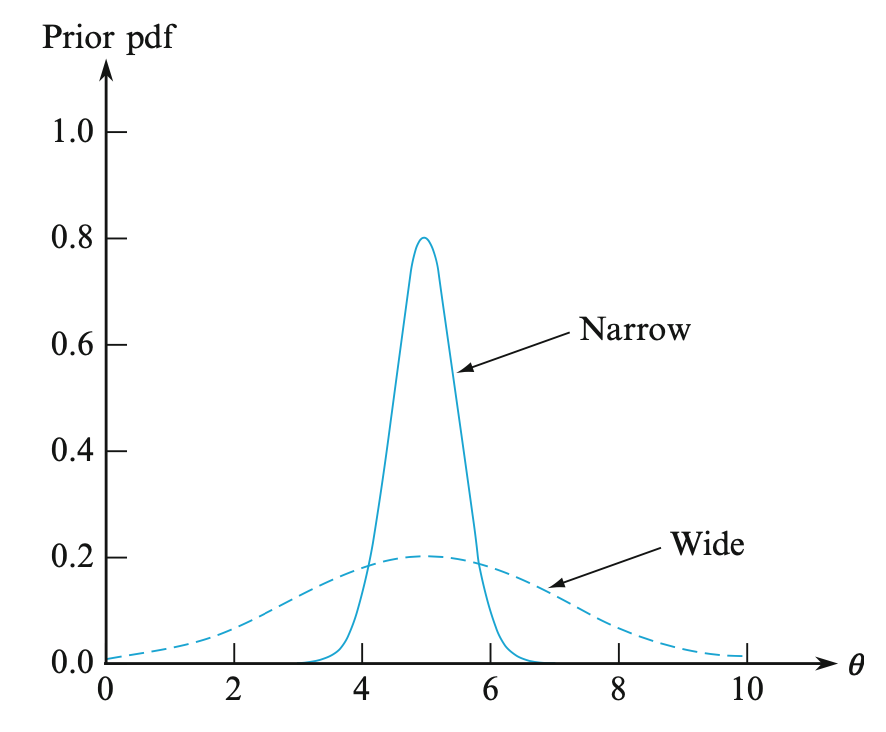
\includegraphics[scale=0.6]{./3_Images/prior_illustration.png}
%    \caption{A narrow concentrated prior about some central value and a wider less informative prior.}
%    \label{fig:prior_illustration}
%    \source{Figure 14.3 in \cite{STK}.}
%\end{figure}


\begin{figure}[H]
    \centering
    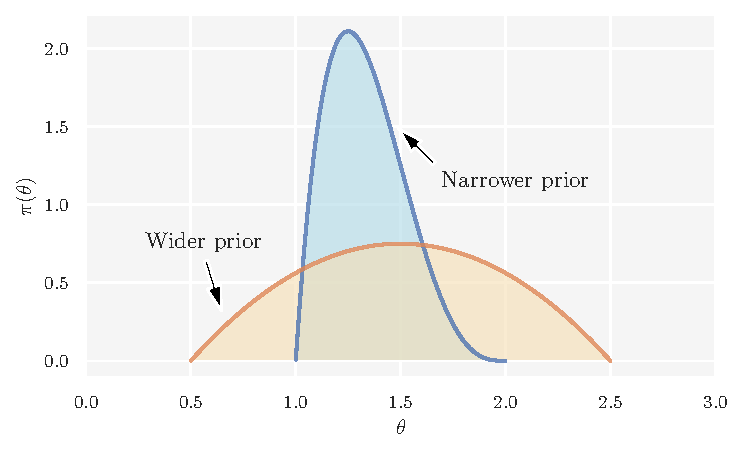
\includegraphics[scale=0.7]{prior_plot}
    \caption{A narrow concentrated prior about some central value and a wider less informative prior.}
    \label{fig:prior_illustration}
    %\source{Figure 14.3 in \cite{STK}.}
\end{figure}

Our prior state of knowledge is modified by data $y$, obtained by performing experiments, through the conditional \textit{sampling distribution} $\lhood$. When regarded as a function of $\theta$, for fixed $y$, $\lhood$ is called the \textit{likelihood function}. In order to make probability statements about $\theta$ given sample data $y$, a probabilistic model representing the joint probability distribution for $\theta$ and $y$ must be provided. The joint pmf or pdf can be written as a product of the prior distribution $\prior$ and the likelihood function $\lhood$:

\begin{equation*}
    \joint = \lhood \prior 
\end{equation*}

At this point, Bayes' theorem is used to produce the \textit{posterior distribution}, which represents our state of knowledge about $\theta$ in the light of $y$. A common incarnation of Bayes' theorem is:

\begin{equation}\label{eq:bayes_theorem}
    \posterior = \frac{\joint}{p(y)}  = \frac{\lhood \prior}{p(y)},
\end{equation}

where the marginal probability of the data $p(y) = \int \lhood \prior \dd \theta$ in the case of continuous parameters, or, in the case of a discrete set of parameters, $p(y) = \sum_\theta \lhood \prior$, where the sum is over all possible values of $\theta$.

$p(y)$ is the same for all possible $\theta$, as it does not depend on $\theta$. With fixed $y$, this factor can thus be omitted in parameter inference since it constitutes a normalizing constant and does not enter into determining the relative posterior probabilities of different values of $\theta$. Omitting the factor $p(y)$ yields the unnormalized posterior distribution: 

\begin{equation}\label{eq:bayes_unnorm}
    \posterior \propto p(\theta, y) =  \lhood \prior 
\end{equation}

In this formulation, $\lhood$ is taken as a function of $\theta$ and not $y$.  

The core of Bayesian inference is encapsulated in \autoref{eq:bayes_theorem} and \autoref{eq:bayes_unnorm}. The principal task is to develop the joint probability model $\joint$ and perform the computations to summarize the posterior $\posterior$.




%================================================================
\subsection{The Prior and Posterior Predictive Distributions}\label{sec:predictive}
%================================================================

BDA, side 7

%================================================================
\section{Summarizing the Posterior}
%================================================================

- mean, median, mode: point estimates

- variance and standard deviation: spread -> uncertainty 

- credible intervals, highest density posterior (hdp) 

%================================================================
\section{Parameter Inference}\label{sec:param_inference}
%\section{Single-parameter Models}\label{sec:single_inference}
%================================================================ 

The way in which Bayes's theorem operates is best seen through examples. 

The way in which Bayes’s theorem operates is best seen through examples. In the following we develop some problem formulations to apply Bayesian analysis on for parameter inference. We will focus on situations where closed forms are available, that is, situations where we can use probability models based on the standard distributions. In particular, we will look at probability models based on the binomial and normal distributions. The binomial distribution is motivated from counting exchangeable outcomes, and the normal distribution applies to a random variable that is the sum of many exchangeable or independent terms. Such models are sometimes unrealistic, but their analysis often provides a useful starting point when it comes to constructing more realistic models. 

The toy problems developed in this section will later serve as benchmark problems. 

%================================================================
%\subsection{The Coin-Flipping Problem}\label{sec:coin_flipping}
\subsection{The Beta-Binomial Model}\label{sec:coin_flipping}
%================================================================ 

The beta-binomial model is one of the simplest interesting Bayesian models, and basic building


Introduce important concepts and computational methods for Bayesian data analysis. 



Every statistics text must contain a coin-flipping example, I'll use it here to get it out of the way. Suppose, naively, that you are unsure about the probability of heads in a coin flip (spoiler alert: it's 50\%). You believe there is some true underlying ratio, call it $p$, but have no prior opinion on what $p$ might be.

We begin to flip a coin, and record the observations: either $H$ or $T$. This is our observed data. An interesting question to ask is how our inference changes as we observe more and more data? More specifically, what do our posterior probabilities look like when we have little data, versus when we have lots of data.

Below we plot a sequence of updating posterior probabilities as we observe increasing amounts of data (coin flips).

It is tractable and easy to extend to more interesting examples

In the simple binomial model, the aim 

The coin-flipping problem, or the beta-binomial model, is a classical problem in statistics where only a single scalar parameter is to be estimated. The problem goes like this


The coin flipping problem, or the beta-binomial model, is a classical problem in statistics and goes like this: 

> We toss a coin a number of times and record how many heads and tails we get. Based on this data, we try to answer questions such as, *is the coin fair*? Or, more generally, *how biased is the coin*? 

In order to estimate the bias of a coin in a Bayesian setting, we will need data and a probabilistic model. For this example, we assume that we have already tossed a coin a number of times and recorded the number of observed heads, so the data-gathering part is already done.

We first generalize the concept of bias. To represent the bias, we will use the $\theta$ parameter. We will say that a coin with $\theta = 1$ will always land heads, one with $\theta=0$ always tails, and one with $\theta=0.5$ will land half of the time heads and the other half tails. We let $y$ represent the total number of heads for a $n$ number of tosses. 


The binomial distribution provides a natural model for data that arise from a sequence of $n$ exchangeable trials or draws from a large population, where each trial gives rise to one of two possible outcomes, conventionally labeled 'success' or 'failure'. Because of the exchangeability, the data can be summarized by the total number of successes in the $n$ trials, which we denote here by $y$. Converting from a formulation in terms of exchangeable trials to one using independent and identically distributed random variables is achieved naturally by letting the parameters $\theta$ represent the proportion of successes in the population or, equivalently, the probability of success in each trial. The binomial sampling model is 

...

where on the left side we suppress the dependence on $n$ because it is regarded as part of the experimental design that is considered fixed; all the probabilities discussed for this problem are assumed to be conditional on $n$.



%================================================================
\section{Toy Problems for Benchmarking}\label{sec:toy_problems}
%================================================================

Develop problems for benchmarking



Only derive this

%================================================================
\subsection{Gaussian Models}\label{sec:gaussian_models}
%================================================================

normal models important blabla

%================================================================
\subsubsection{With Unknown Mean}
%================================================================

The comprehensive derivation can be found in appendix B. 

Devore, p. 781 

Note that the posterior mean $\mu_0'$ is a weighted average of the prior mean $\mu_0$ and the data mean $\bar{x}$, with weights that are the reciprocals of the prior variance and the variance of $\bar{x}$. It makes sense to define the \textbf{precision} as the reciprocal of the variance because a lower variance implies a more precise measurement and the weights then are the corresponding precisions. Furthermore, the posterior variance is the reciprocal of the sum of the reciprocals of the two variances, but this can be described much more simply by saying that the posterior precision is the sum of the prior precision plus the precision of $\bar{x}$. 

%================================================================
\subsubsection{With Unknown Variance}
%================================================================

The comprehensive derivation can be found in appendix B. 

%================================================================
\subsubsection{With Unknown Mean and Variance}
%================================================================

The comprehensive derivation can be found in appendix B. 




%================================================================
\section{The Influence of the Prior and How to Choose One}\label{sec:prior}
%================================================================

\begin{itemize}
    \item Flat
    \item Uninformative
    \item Diffuse
    \item The Jeffreys’ Prior: Suppose we cannot easily find the natural scale on which the likelihood is in data-translated format, or that such a decomposition does not exist. Jeffreys (1961) proposed a general prior in such cases, based on the Fisher information I of the likelihood. 
    \item When a prior distribution is not integrable it is said to be \textit{improper}
\end{itemize}


%================================================================
\subsection{Conjugate Prior Distributions}
%================================================================

Conjugacy is formally defined as follows. If $\mathcal{F}$ is a class of sampling distributions $p \left(y | \theta \right)$, and $\mathcal{P}$ is a class of prior distributions for $\theta$, then the class $\mathcal{P}$ is \textit{conjugate} for $\mathcal{F}$ if

\begin{equation}
    \pi \left(\theta | y \right) \in \mathcal{P} \, \forall p \left(\cdot | \theta \right) \in \mathcal{F} \land \pi (\cdot) \in \mathcal{P}
\end{equation}

This definition is formally vague since if we choose $\mathcal{P}$ as the class of all distributions, then $\mathcal{P}$ is always conjugate no matter what class of sampling distributions is used. We are most interested in \textit{natural} conjugate prior families, which arise by taking $\mathcal{P}$ to be the set of all densities having the same functional form as the likelihood \cite{ABC_ch1}.

A conjugate prior of a likelihood is a prior that, when used in combination with a given likelihood, returns a posterior with the same functional form as the prior. cite BAP

%================================================================
\section{Prior and Posterior Predictive Checks}
%================================================================

\begin{itemize}
    \item \url{https://docs.pymc.io/notebooks/posterior_predictive.html}
    \item \url{https://avehtari.github.io/masterclass/slides_ppc.pdf}
    \item \url{https://vasishth.github.io/bayescogsci/book/sec-priorpred.html}
    \item \url{https://betanalpha.github.io/assets/case_studies/principled_bayesian_workflow.html#113_Prior_Predictive_Checks}
    \item \url{http://bebi103.caltech.edu.s3-website-us-east-1.amazonaws.com/2018/tutorials/t6a_model_generation_and_prior_predictive_checks.html} python
\end{itemize}

%================================================================
\section{Uncertainty/Sensitivty Analysis in the Bayesian Paradigm}
%================================================================

TODO

\section{Topics} 

In Bayesian inference, posterior beliefs about parameters are updated according to \textit{Bayes' theorem} upon observing data.  

The mean of this posterior distribution gives a point estimate of $\theta$. 

An interval having a posterior probability $.95$ gives a $95\%$ \textit{credibility} interval, an interval within which an unobserved parameter value falls with a particular probability, the Bayesian analogue of a $95\%$ confidence interval \cite[p. 777]{STK}.

Credible intervals 

HDI 

Energy


%================================================================
\section{Why Bayes?}
%================================================================

End chapter with this?
